\tightsection{Improving Quality with GO}
\label{sec:improvement}

Previous sections have established our prediction algorithm can achieve low prediction accuracy. In this section, we empirically study if a good prediction lead to high improvement. It should be noticed that the possible improvement is bounded by the actual difference between the performance of resources (e.g., CDN or bitrate). As pointed out in \Section~\ref{sec:intro}, current industrial practice however, only allows coarse grain decisions (e.g., inter-CDN selection) and the difference at such level is much less significant than finer-grain ones (e.g., server selection or even path selection). Therefore, though based on our dataset our quantitative results do not show remarkable improvement under CDN or bitrate selection, we expect to see higher improvement with more fine-grain selection enabled and thus larger room of improvement.

Specifically, we aim to answer three questions:
\begin{packedenumerate}
	\item How does GO select best decision based on prediction (\Section~\ref{subsec:behavior})?
	\item How much quality improvement can GO achieve (\Section~\ref{subsec:go-improve})?
	\item How much do different factors (e.g., prediction accuracy and quality diversity) impact quality improvement (\Section~\ref{subsec:impact-accuracy} and ~\ref{subsec:impact-diversity})?
\end{packedenumerate}

\tightsubsection{Methodology \jc{This part must be shrinked}}
We study these questions by using offline trace-driven analysis. As we will introduce in \Section~\ref{sec:eval}, we have built GO system that runs in real world, and we use real world experiments to demonstrate GO's behavior and its quality improvement in the wild. However, we believe these questions should be better addressed using offline trace-driven analysis due to its flexibility in following four dimensions.
\begin{packedenumerate}
	\item More overage: The real world experiments only have access to the video traffic of one video site on one type of OS with one streaming protocol. The greatly constraints its coverage on types of traffic.
	\item More scale of simultaneous expriments: The real world experiment only controls one site's traffic, it is infeasible to compare a lot of configurations or algorithms in parallel (empirically, at most 3-4) and ensure each of them receive sufficient traffic to draw confident conclusions.
	\item More diversity in performance: As we will see, quality improvement is greatly impacted by the diversity in the performance outcome among different decisions (e.g., different CDNs). However, we can only observe a limited number of possible patterns of performance diversity in real world expreiments.
	\item More controlled experiments: It is also impossible to conduct sensitivity analysis (e.g., the third question) where we would lik to change one parameter (e.g., CDN performance) at a time with a controlled amount.
\end{packedenumerate}


This section uses three input to answer the two high-level questions. We now describe them in the order of closeness to realism and in reverse order of degree of controllability.

\myparatight{Counterfactual input} This approach is the closest to real-world experiment. The basic idea is that we first collect a dataset in which the decisions are randomly made for each client (called {\it random dataset}) and collect the quality metrics of each video session under random decisions. Then we evaluate a given decision algorithm by picking the sessions for which the decision made by the algorithm matches the decisions in the random dataset. In~\cite{technicalreport}, we show that this approach is unbiased. 
By using this methodology, we are able to replay multiple algorithms on the data sets.

\myparatight{Augmented trace-driven input} While counterfactual input is useful in evaluating different algorithms, we cannot use it to estimate the ``would-be" performance of an ``oracle" approach (e.g., how the performance would be if another decision were taken), which requires data extrapolation. To remedy these limitations, we generate an augmented trace-driven synthetic dataset in which we extrapolate for each session the ``true'' quality outcome of all its possible decisions. The basic idea of this extrapolation  is that for each session $s$, its outcome of each decision $d$ is drawn from the distribution of outcomes of this decision on other sessions exactly matching the same attributes with $s$. Having ensured that quality outcomes in the synthetic scenario are known for any decision, it is possible to identify an {\it oracle} approach that always makes the best decision. However, the evaluation is may possibly be biased by the extrapolation.

\myparatight{Controlled synthetic input} Both previous methodology lacks control, i.e., if no major outage or other events happen in the data set, we cannot evaluate GO performance under those scenarios. Thus we also use fully controlleable input in which the true outcomes (i.e., ``ground truth'') of each decision is controlled.


\tightsubsection{A Simple Example}
\label{subsec:behavior}

We first explain the GO's prediction-based decision making and use controlled synthetic input to confirm its behavior -- GO identifies the performance changes and switches decision accordingly if needed.

\myparatight{Prediction-based dececision making} When selecting decisions, GO simply selects for each session under prediction the decision that has the best predicted quality in a certain metric. Note that GO always leaves a small fraction of traffic to be randomly allocated to guarantee that each decision will have at least certain fraction of traffic even when that decision is not the best for every session at this point (but potentially, the best in the future).


\begin{figure}[h!]
\centering
 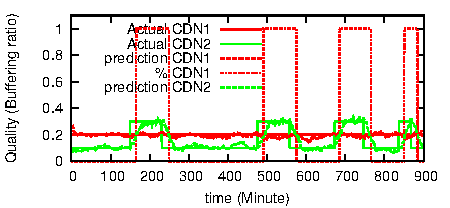
\includegraphics[width=0.5\textwidth] {figures/behavior-evaluation/simple-change.pdf}
\tightcaption{Case for behavioral study}
\label{fig:behavioral}
\end{figure}

\myparatight{Case study} We simulate a scenario in which a sudden change in performance of one group causes GO to switch decision accordingly. Figure~\ref{fig:behavioral} shows the behavior of sessions in one ASN when provided with two CDNs to choose from. We only use buffering ratio as quality metric. The mean of buffering ratio of CDN1 is stably at 0.2 and that of CDN2 changes between 0.1 and 0.25, with a random interval. Each quality sample of a CDN is generated so that its buffering ratio has a Guassian noise with standard deviation of 0.01 from mean. This figure shows clearly that under this configuration, GO is able to switch to the best CDN accordingly with an expected delay (as it uses a 30-minute sliding window). Note that there is always a small amount of randomized traffic, so the change on each decision can be detected. %As a side-effect, it takes longer for GO to detect that CDN2 has bad bad quality than when it has good quality, because the number of samples from CDN2 when it has bad quality (only randomized traffic) is smaller than when it has good quality (all traffic).

%\xil{are we going to do something about that point or ack it is an issue.}



\tightsubsection{Evaluation of Quality Improvement}
\label{subsec:go-improve}

We define quality improvement over a set of sessions in two measures: improvement ratio and optimality, which are defined as follows.

\begin{align*}
& ImprovemenRatio=\frac{Q_{GO}-Q_{Baseline}}{Q_{Baseline}}\\
& Optimality=\frac{Q_{Oracle}-Q_{Baseline}}{Q_{GO}-Q_{Baseline}}
\end{align*}

Here, $Q$ is the average quality of these sessions. Oracle means to select the best decision based on its true outcome, so the it is only available in augmented trace-driven input and controlled synthetic input.  By default, we use random selection as the baseline which always select a uniformly random decision among all possible ones. Improvement ratio is larger the better and optimality is closer to one the better.


We use counterfactual input to evaluate GO's improvement ratio. Figure~\ref{fig:cross-metrics} shows the improvement ratio on each metric when GO uses different metrics as utility function (i.e., GO makes decision based on the predicted quality of different decisions on this metric). From the figure, we find that the largest improvement happens when GO uses the same metric to be utility function as the one we evaluate it. Surprisingly, we also see arguable improvement on other metrics when they are not explicitly optimized. For example, by using metrics other than average bitrate as utility function, we can still achieve 2\%-25\% improvement in average bitrate.


\begin{figure}[h!]
\centering
 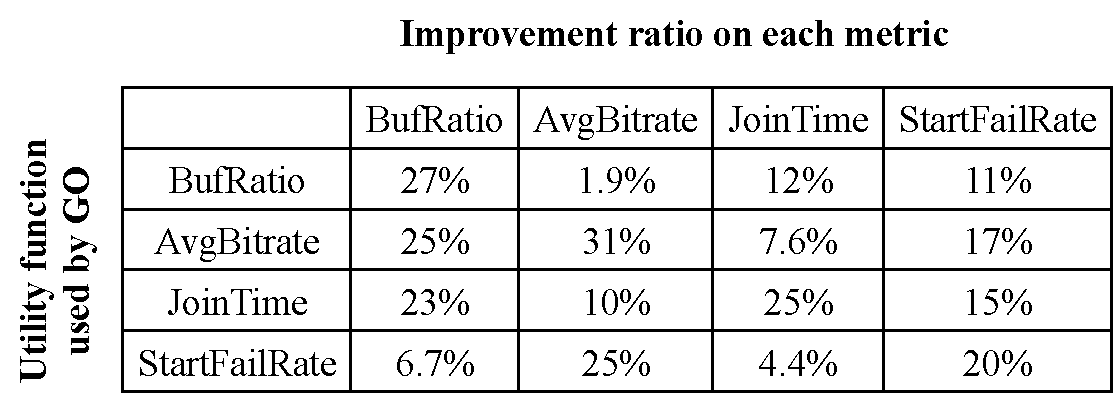
\includegraphics[width=0.45\textwidth] {figures/newfig/cross-metric.pdf}
\tightcaption{Improvement ratio on each metric by using different metric as utility function.}
\label{fig:cross-metrics}
\end{figure}


\tightsubsection{Sensitivity Analysis}

\tightsubsubsection{Impact of Prediction Accuracy}
\label{subsec:impact-accuracy}

To quantify the impact of prediction accuracy, we use the augmented trace-driven testing since we need the true quality so that we can controll prediction error. We change GO's prediction error and evaluate the improvement ratio and optimality. 


We use the augmented trace-driven testing to control the prediction error and quantify its impact on quality improvement. Given a session and one decision, if the true quality is $q$ and $p$ is the prediction made by GO, we use a parameter called stretch ratio $r_a$ to change the prediction $p$ to new prediction $p'=q+(p-q)r_a$ so that the prediction error is exactly stretched by $r_a$. 
In addition, we compare with an oracle which always makes the best decision based on true quality of each decision. To simplify the discussion, we assume each session has two  possible decisions. 

\begin{figure}[h!]
\centering
 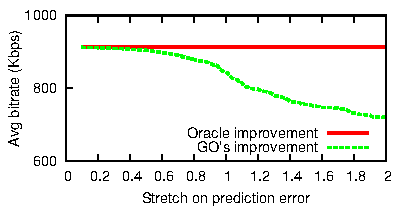
\includegraphics[width=0.35\textwidth] {figures/newfig/trendAccuracy-metricId1-keyGlobal-partition.pdf}
\tightcaption{Impact of GO prediction accuracy with varying stretch ratio $r_a$ on quality improvement.}
\label{fig:trace-accuracy-2}
\end{figure}

Figure~\ref{fig:trace-accuracy-2} shows GO's improvement ratio when average bitrate is used as utility function and evaluated metric.
It shows a clear degredation in improvement ratio. When stretch ratio is close to zero, GO gives perfect prediction and thus GO gives the same quality as the oracle (i.e., GO's optimality is one). With stretch ratio larger than 0.7, every 10\% decrease in prediction error gives 20Kbp increase in improvement ratio of average bitrate. It suggests that the improvement is sensitive to accuracy -- if current prediction error is reduced by 30\%, GO will have 12.5\% more improvement. 
%Also, note that with smaller stretch rate, the improvement stablizes as the improvement converges to oracle improvement with accurate prediction.



\tightsubsubsection{Impact of Quality Diversity}
\label{subsec:impact-diversity}

To quantify the impact of quality diversity among multiple decisions, we fix the prediction error given by GO, and use a stretch ratio $r_b$ to control the quality diversity between multiple decisions. To simplify the discussion, we again assume each session has two possible decisions. Given a session with the true quality of two decisions being $q_1, q_2$ (assume $q_1\leq q_2$), we change their value to $q_1'=q_1, q_2=q_1+(q_2-q_1)r_b$. We show quality improvement in absolute number over the baseline algorithm, as well as the optimality.

%Intuitively, it is expected that with larger quality diversity among multiple decisions, we should see that GO's performance should be closer to the oracle approach since the gap between decisions' outcome is so large that the best decision will be made with any prediction error. 

\begin{figure}[h!]
\centering
\subfigure[Average bitrate (Kbps)]
{
        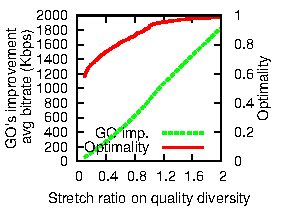
\includegraphics[width=0.24\textwidth]{figures/newfig/trendDiversity-metricId1-keyGlobal-partition.pdf}
}
\hspace{-0.6cm}
\subfigure[Join time (ms)]
{
        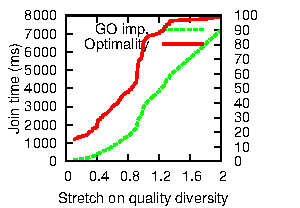
\includegraphics[width=0.24\textwidth]{figures/newfig/trendDiversity-metricId2-keyGlobal-partition.pdf}
}
\tightcaption{Impact of stretch of quality diversity $r_b$ on quality improvement. Green lines with values on the left y axis show GO's improvement over the randomized baseline and red lines with values on the right y axis show optimality (GO's improvement/oracle's improvement)}
\label{fig:trace-diversity}
\end{figure}

Figure~\ref{fig:trace-diversity} shows the result with average bitrate and join time as the utility function and evaluation metrics. The left y axis shows the improvement of GO. In both figures, they show a close-to-linear relationship between improvement and quality diversity among decisions. 
The right y axis gives the optimality. Both figures show that when the diversity increases for 100\%, GO will give almost the same improvement as oracle approach. 



\tightsubsection{Summary of Findings}
\begin{packedenumerate}
	\item Under controlled experiments, GO identifies performance change and switches decisions accordingly.
	\item GO achieves noticeable improvement on four metrics, e.g., for buffering ratio, 1.5\% globally and as much as 4.8\% for some popular site.
	\item Optimizing for one metric does not impact other metric negatively. Instead, we see improvement on all metrics if only one metric is used for decision selection.
	\item Quality improvement is linear to prediction error -- 10\% reduction in prediction error yields to 20Kbps in average bitrate improvement, and if current prediction error is reduced by 30\%, GO will have 12.5\% more improvement in average bitrate.
	\item GO's quality improvement in average bitrate increases almost linearly with quality diversity between decisions, and such improvement becomes closer-to-optimal with larger quality diversity -- if the current quality difference increases by 50\%, GO can achieve improvement in join time as much as 90\% of the optimal improvement.
\end{packedenumerate}


